\section{Muon Momentum Resolution}

High-Pt muons ($P_{t}>200GeV$) suffer from high energy loss by travelling in Iron
due to radiative processes. The transverse momentum measurement relays on
sagita ($s \propto 1/Pt$) which is associated with the number of hits found on
the Tracker and the Muon systems. As the number of hits is lower on the so called
tracker muons, i.e muons that were reconstructed from hits in the tracker and the
first statition of the muon sistem, a study is needed to determine
the resolution of this Pt measurement for tracker-HighPt ID muons.

\begin{sidewaystable}[htb]
\begin{center}
  \caption{Montecarlo Samples used to study the Muon Momentum Resolution}
\footnotesize
\begin{tabular}{|l|l|l|}
\hline
Year & Sample & XSec [pb] \\ \hline
\hline
2016 & ZToMuMu\_NNPDF30\_13TeV-powheg\_M\_50\_120 & 2.116e+03\\
&ZToMuMu\_NNPDF30\_13TeV-powheg\_M\_120\_200 & 2.058e+01\\
&ZToMuMu\_NNPDF30\_13TeV-powheg\_M\_200\_400 & 2.890e+00\\
&ZToMuMu\_NNPDF30\_13TeV-powheg\_M\_400\_800 & 2.515e-01\\
&ZToMuMu\_NNPDF30\_13TeV-powheg\_M\_800\_1400 & 1.709e-02\\
&ZToMuMu\_NNPDF30\_13TeV-powheg\_M\_1400\_2300 & 1.370e-03\\
&ZToMuMu\_NNPDF30\_13TeV-powheg\_M\_2300\_3500 & 8.282e-05\\
&ZToMuMu\_NNPDF30\_13TeV-powheg\_M\_3500\_4500 & 3.414e-06\\
&ZToMuMu\_NNPDF30\_13TeV-powheg\_M\_4500\_6000 & 3.650e-07\\
&ZToMuMu\_NNPDF30\_13TeV-powheg\_M\_6000\_Inf & 2.526e-08\\
\hline
2017 & ZToMuMu\_NNPDF31\_TuneCP5\_13TeV-powheg-pythia8\_M\_50\_120 & 2.116e+03\\
&ZToMuMu\_NNPDF31\_TuneCP5\_13TeV-powheg-pythia8\_M\_120\_200 & 2.058e+01\\
&ZToMuMu\_NNPDF31\_TuneCP5\_13TeV-powheg-pythia8\_M\_200\_400 & 2.890e+00\\
&ZToMuMu\_NNPDF31\_TuneCP5\_13TeV-powheg-pythia8\_M\_400\_800 & 2.515e-01\\
&ZToMuMu\_NNPDF31\_TuneCP5\_13TeV-powheg-pythia8\_M\_800\_1400 & 1.709e-02\\
&ZToMuMu\_NNPDF31\_TuneCP5\_13TeV-powheg-pythia8\_M\_1400\_2300 & 1.370e-03\\
&ZToMuMu\_NNPDF31\_TuneCP5\_13TeV-powheg-pythia8\_M\_2300\_3500 & 8.282e-05\\
&ZToMuMu\_NNPDF31\_TuneCP5\_13TeV-powheg-pythia8\_M\_3500\_4500 & 3.414e-06\\
&ZToMuMu\_NNPDF31\_TuneCP5\_13TeV-powheg-pythia8\_M\_4500\_6000 & 3.650e-07\\
&ZToMuMu\_NNPDF31\_TuneCP5\_13TeV-powheg-pythia8\_M\_6000\_Inf & 2.526e-08\\
\hline
2018 & ZToMuMu\_NNPDF31\_TuneCP5\_13TeV-powheg-pythia8\_M\_50\_120 & 2.116e+03\\
&ZToMuMu\_NNPDF31\_TuneCP5\_13TeV-powheg-pythia8\_M\_120\_200 & 2.058e+01\\
&ZToMuMu\_NNPDF31\_TuneCP5\_13TeV-powheg-pythia8\_M\_200\_400 & 2.890e+00\\
&ZToMuMu\_NNPDF31\_TuneCP5\_13TeV-powheg-pythia8\_M\_400\_800 & 2.515e-01\\
&ZToMuMu\_NNPDF31\_TuneCP5\_13TeV-powheg-pythia8\_M\_800\_1400 & 1.709e-02\\
&ZToMuMu\_NNPDF31\_TuneCP5\_13TeV-powheg-pythia8\_M\_1400\_2300 & 1.370e-03\\
&ZToMuMu\_NNPDF31\_TuneCP5\_13TeV-powheg-pythia8\_M\_2300\_3500 & 8.282e-05\\
&ZToMuMu\_NNPDF31\_TuneCP5\_13TeV-powheg-pythia8\_M\_3500\_4500 & 3.414e-06\\
&ZToMuMu\_NNPDF31\_TuneCP5\_13TeV-powheg-pythia8\_M\_4500\_6000 & 3.650e-07\\
&ZToMuMu\_NNPDF31\_TuneCP5\_13TeV-powheg-pythia8\_M\_6000\_Inf & 2.526e-08\\
\hline
\end{tabular}
\label{tab:MomentumResolutionSamples}
\end{center}
\end{sidewaystable}

The momentum resolution can be defined as a relative difference between the
momentum reconstructed and the true momentum from monte carlo simulations.

\begin{equation}
\frac{P_{GEN}}{P_{RECO}} - 1 = \frac{\dfrac{1}{P_{RECO}}-\dfrac{1}{P_{GEN}}}{\dfrac{1}{P_{RECO}}}
\end{equation}

These studies were performed by simulating the standard model Z boson production
decaying to a pair of Muons ($Z\rightarrow\mu\mu$) the complete list of samples is
provided on table \ref{tab:MomentumResolutionSamples}
Z-Mass binned samples were used in order to increase the number of available
statistics in a wide range of transverse momentum, specially on the High-Pt sector.

\begin{figure}[tph]
  \centering
  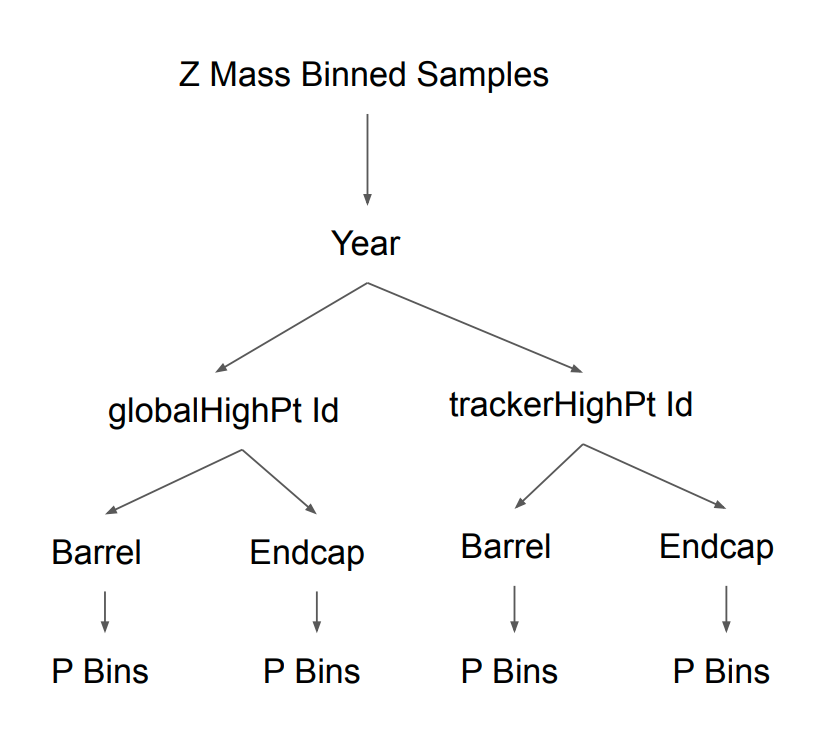
\includegraphics[width=.5\textwidth]{fig/MomentumResolution/MomentumResolutionBins.png}
  \caption{Signal efficiency for individual and combined High Level Triggers for Run II}
  \label{fig:MomentumResolutionBins}
\end{figure}

A counting experiment following the trigger and muon selection described on
section %\ref{}%
collects the momentum resolution for each indivual Muon which is then classified
on different bins depending on its ID, either global or tracker High-Pt; the $\eta$
region in the Muon detector, i.e the barrel ($\lvert eta\lvert< 1.2$) or
the endcap ($1.2 < \lvert eta \lvert < 2.4$); and its transverse momentum range
(see figure \ref{fig:MomentumResolutionBins}).


\begin{figure}[tph]
  \centering
  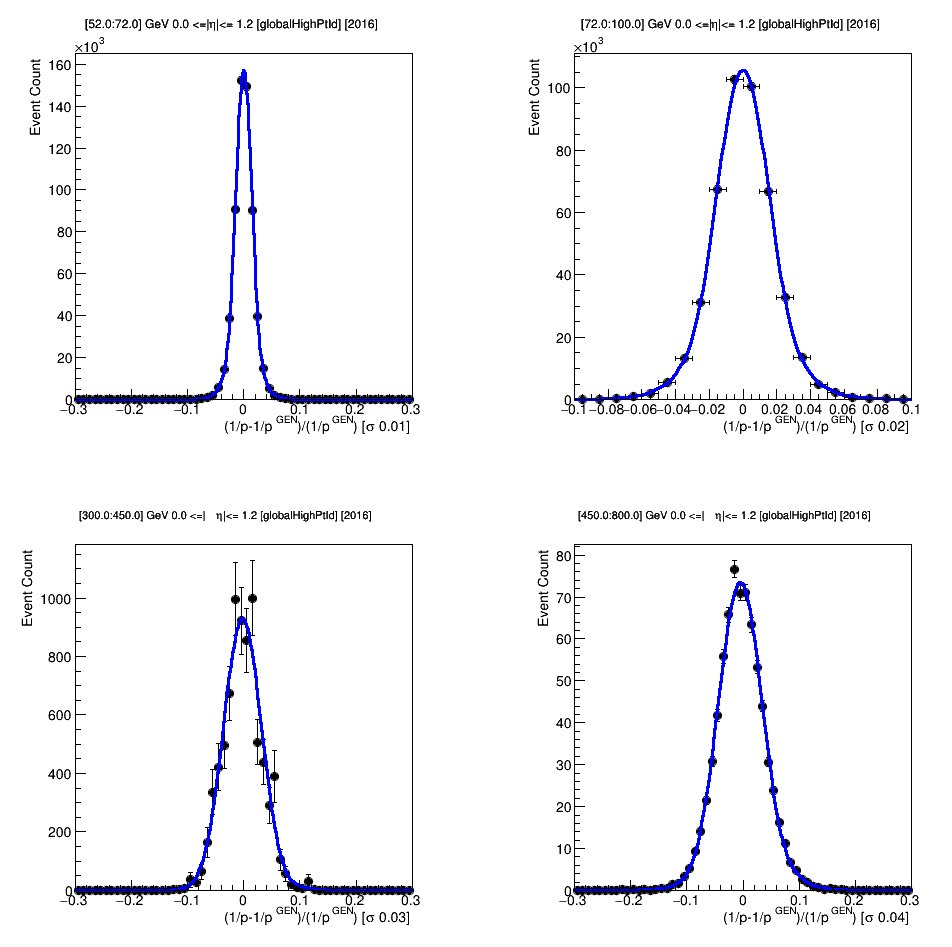
\includegraphics[width=.7\textwidth]{fig/MomentumResolution/DSCB_Example.png}
  \caption{
    The Double-Sided Crystall Ball fit is shown as the blue solid line,
    the number of events as counted from MC samples are shown in black markers for
    the momentum resolution. The example shows the 2016 samples for muons labeled
    as globalHigh-Pt, seen in the barrel of the muon system. Different momentum
    ranges are shown, the
    top-left figure shows muons with momentum in the range $[52:72]~GeV$,
    the top-right figure $[72:100]~GeV$, bottom-left $[300:450]~GeV$,
    bottom-right $[450:800]~GeV$. The value for the width $\sigma$ for the DSCB
    distribution is shown on the horizontal axis and it shows evidence of how
    the resolution increases as the momentum range gets higher.
  }
  \label{fig:DSCB_Fit_Example}
\end{figure}

The distribution is then fitted by using a Double-Sided Crystall Ball (DSCB)
(\verb|RooCrystalBall| in \verb|RooFit|) which is a distribution defined
by parts, with a range-limited gaussian form around its mean with two
exponential tails which help model the nature of radiative processes occurring in
the detector. The width of the gaussian portion of the DSCB provides the
resolution (as a percentage) while the mean accounts for any bias present on the
momentum measurements. An example of the fit is shown in \ref{fig:DSCB_Fit_Example}

\subsection{Z-Mass Resolution}

\begin{sidewaystable}[htb]
\begin{center}
  \caption{Montecarlo Samples for Z Mass Resolution studies}
\footnotesize
\begin{tabular}{|l|l|l|}
\hline
Year & Sample & XSec [pb] \\ \hline
\hline
2016 & DYJetsToMuMu\_M-50\_Zpt-150toInf\_TuneCP5\_13TeV-madgraphMLM\_pdfwgt\_F-pythia8 & 6.178e+00\\
\hline
2017 & DYJetsToMuMu\_M-50\_Zpt-150toInf\_TuneCP5\_13TeV-madgraphMLM\_pdfwgt\_F-pythia8 & 6.182e+00\\
\hline
2018 & DYJetsToMuMu\_M-50\_Zpt-150toInf\_TuneCP5\_13TeV-madgraphMLM\_pdfwgt\_F-pythia8 & 6.178e+00\\
\hline
\end{tabular}
\label{tab:ZMassResolutionSamples}
\end{center}
\end{sidewaystable}
